\section{Технический проект}
\subsection{Общая характеристика организации решения задачи}

В рамках решения задачи цифровизации туристической инфраструктуры региона была разработана концепция веб-приложения, ориентированного на широкую аудиторию — как местных жителей, так и туристов. Основной целью проекта стало создание удобной цифровой среды, позволяющей пользователю оперативно получать информацию о достопримечательностях, прокладывать маршруты и формировать персонализированные планы посещения.

Организация решения строится на модульном подходе\cite{b12}, при котором система разбивается на взаимосвязанные, но относительно независимые компоненты: модуль работы с картой, система фильтрации и поиска объектов, маршрутный модуль, интерфейс взаимодействия с пользователем, а также серверная логика, обеспечивающая хранение и обработку данных. Такое разделение упрощает поддержку и масштабирование проекта, позволяя в будущем дополнять его новыми возможностями без необходимости полной переработки архитектуры.

Веб-приложение функционирует в клиент-серверной модели\cite{b13}. Клиентская часть обеспечивает визуализацию данных, управление маршрутом и взаимодействие с картой, а серверная часть отвечает за хранение пользовательской информации, логирование действий, выдачу данных о туристических объектах, а также обработку маршрутов. Обмен между клиентом и сервером реализуется через REST API с использованием формата JSON, что обеспечивает гибкость и универсальность взаимодействия.

Информационное наполнение веб-приложения формируется из предварительно структурированных данных о достопримечательностях региона. Каждая точка интереса включает в себя географические координаты, категорию, краткое описание, изображения, а также дополнительные атрибуты, позволяющие фильтровать объекты по предпочтениям пользователя. Данные хранятся в базе, доступ к которой осуществляется с учётом требований безопасности и производительности.

\subsection{Обоснование выбора технологии проектирования}

Выбор технологий для реализации веб-приложения, посвящённого цифровой навигации по туристическим объектам региона, основывался на совокупности факторов: масштаб проекта, тип данных (в том числе геолокационных), необходимость интерактивного интерфейса и перспектива последующего расширения функционала. Особое внимание уделялось поддержке адаптивности, производительности и удобству взаимодействия с картографическими сервисами.

\subsubsection{Описание используемых технологий и языков программирования}

В процессе разработки web-сайта используются программные средства и языки программирования. Каждое программное средство и каждый язык программирования применяется для круга задач, при решении которых они необходимы.

\subsubsection{Язык разметки HTML}

HTML (HyperText Markup Language) — это стандартный язык разметки\cite{b19}, используемый для создания структуры веб-страниц. Он задаёт расположение и тип элементов интерфейса: заголовков, абзацев, кнопок, форм, списков и других компонентов. В рамках данного проекта HTML используется для:
\begin{itemize}
	\item определения компоновки интерфейса веб-приложения (например, блок карты, меню фильтров, карточки объектов);
	\item разметки форм маршрута, поиска и фильтрации точек интереса;
	\item обеспечения семантики, что повышает доступность и SEO-оптимизацию проекта;
	\item интеграции с JavaScript и стилями (CSS) — через идентификаторы, классы и атрибуты.
\end{itemize}

Благодаря чистой и логичной HTML-разметке упрощается последующее стилизование и взаимодействие с элементами через скрипты.

\subsubsection{Язык стилей CSS}

CSS используется для визуального оформления элементов, определения расположения блоков, выбора шрифтов, цветов и адаптации интерфейса под различные устройства. В проекте применяются:
\begin{itemize}
	\item анимации и визуальные эффекты для плавного появления элементов, наведения на кнопки и взаимодействия с маршрутом на карте;
	\item стилизация форм (полей ввода, выпадающих списков), карточек достопримечательностей, балунов карты и навигационных элементов.
\end{itemize}

CSS играет ключевую роль в восприятии системы конечным пользователем, обеспечивая привлекательность и удобство интерфейса.

\subsubsection{Язык программирования JavaScript}

JavaScript\cite{b18} — это язык программирования, который используется для добавления интерактивности на веб-страницах. Он позволяет обрабатывать действия пользователя, изменять элементы интерфейса без перезагрузки страницы и взаимодействовать с сервером. В проекте он используется для:
\begin{itemize}
	\item реализации фильтрации объектов в реальном времени без перезагрузки страницы;
	\item динамического добавления, удаления и сортировки точек маршрута;
	\item обработки кликов по карте, открытия балунов, взаимодействия с API Яндекс.Карт;
	\item обновления интерфейса в ответ на действия пользователя (например, отображение построенного маршрута, переключение категорий, переход между вкладками);
	\item отправки запросов к серверу и получения данных (API);
	\item управления состоянием интерфейса (например, сохранение списка избранного или выбранного типа маршрута).
\end{itemize}

JavaScript позволяет превратить статичную HTML-разметку в полноценное интерактивное приложение.

\subsubsection{Язык программирования PHP}

PHP — это язык серверной логики, работающий на стороне сервера. Он отвечает за обработку пользовательских запросов, взаимодействие с базой данных, управление сессиями и генерацию динамического HTML. Основные задачи PHP в рамках проекта:
\begin{itemize}
	\item формирование API-эндпоинтов для получения информации о точках интереса, маршрутах, пользователях;
	\item обработка входящих запросов: фильтрация, валидация, авторизация;
	\item хранение, обновление и удаление данных в базе;
	\item обеспечение безопасности;
	\item регистрация и авторизация пользователей, управление сессиями.
\end{itemize}

PHP, благодаря своей простоте и зрелой экосистеме, позволяет реализовать устойчивую и надёжную серверную часть с широкими возможностями по расширению.

\subsubsection{API Яндекс.Карт}

Яндекс.Карты API — это программный интерфейс, предоставляемый Яндексом для работы с их картографическим сервисом. Позволяет отображать интерактивные карты, добавлять метки, строить маршруты, использовать геолокацию и геокодинг.

Картографическое API Яндекс.Карт является ключевым компонентом проекта, обеспечивая визуальное отображение туристических объектов и построение маршрутов. Основные его функции в приложении:
\begin{itemize}
	\item отображение карты региона — с возможностью приближения, переключения слоёв и центрирования;
	\item добавление кастомных меток — каждая достопримечательность отображается своей иконкой, имеет всплывающий балун с описанием и кнопками действий;
	\item построение маршрутов — между произвольным количеством точек, включая начальную, конечную и промежуточные;
	\item кластеризация точек — при большом количестве объектов на карте они группируются в кластеры, упрощая восприятие;
	\item фильтрация и управление слоями — отображение только выбранных категорий (музеи, архитектурные объекты, природные и др.);
	\item интерактивность — пользователь может кликать по карте, добавлять точки маршрута, просматривать подробную информацию.
\end{itemize}

Использование Яндекс.Карт оправдано не только их функциональностью, но и точной локализацией и высокой детализацией регионов России, включая Курскую область.

\subsection{Архитектура программной системы}

Пользователь через браузер (клиентскую часть) отправляет запрос на построение маршрута. Этот запрос обрабатывается сервером Nginx и перенаправляется на PHP-приложение, которое обращается к базе данных\cite{b14} для получения информации об объектах, после чего строит маршрут с помощью API Яндекс.Карт. Готовый результат отправляется обратно пользователю в виде визуализации на карте и текстовых подсказок.

Программная система состоит из следующих компонентов:
\begin{enumerate}
	\item  Клиентская часть (Frontend). В основе клиентской части лежит набор веб-технологий, включая HTML, CSS и JavaScript. Эти технологии формируют пользовательский интерфейс, обеспечивающий визуальное взаимодействие с системой. HTML используется для структурирования содержимого страниц, CSS — для оформления и адаптации интерфейса под различные устройства, а JavaScript обеспечивает интерактивность. Например, действия пользователя, такие как выбор категории достопримечательностей или построение маршрута, обрабатываются с помощью JavaScript, который динамически обновляет содержимое без необходимости полной перезагрузки страницы. Отображение карты и точек на ней реализовано через подключение JavaScript-библиотеки Яндекс.Карт, позволяющей накладывать пользовательские метки, маршруты и настраивать поведение интерфейса карты.
	\item Промежуточный сервер (Web Server). Между клиентом и сервером располагается прокси-сервер, который выполняет роль маршрутизатора. Он принимает все входящие HTTP-запросы, обрабатывает их на начальном уровне (например, применяет HTTPS-шифрование, фильтрует запросы и кеширует часто используемые ресурсы), а затем перенаправляет их на сервер приложений. Такая прослойка значительно повышает производительность и безопасность системы.
	\item Сервер приложений (Backend). На серверной стороне работает программная логика, написанная на PHP. Здесь происходит основная обработка данных. Когда пользователь, например, строит маршрут между двумя туристическими объектами, PHP-скрипты получают данные о начальной и конечной точке, выполняют проверку и, при необходимости, обращаются к API Яндекс.Карт для получения оптимального маршрута. PHP также взаимодействует с базой данных, в которой хранятся сведения обо всех достопримечательностях, пользователях, отзывах, избранных местах и сохранённых маршрутах.
	\item Внешние API. Важным элементом архитектуры является использование внешних API. Центральное место здесь занимает API Яндекс.Карт, который обеспечивает не только отображение карты, но и функционал геокодирования (преобразование адресов в координаты), построение маршрутов с различными параметрами (пешком, на машине, на общественном транспорте) и вывод вспомогательных подсказок. Благодаря этому API веб-приложение получает возможность предоставить пользователю высокоинтерактивную карту с широкими возможностями.
\end{enumerate}

На рисунке \ref{data:image} представлена архитектура программной системы.

\begin{figure}[ht]
	\center{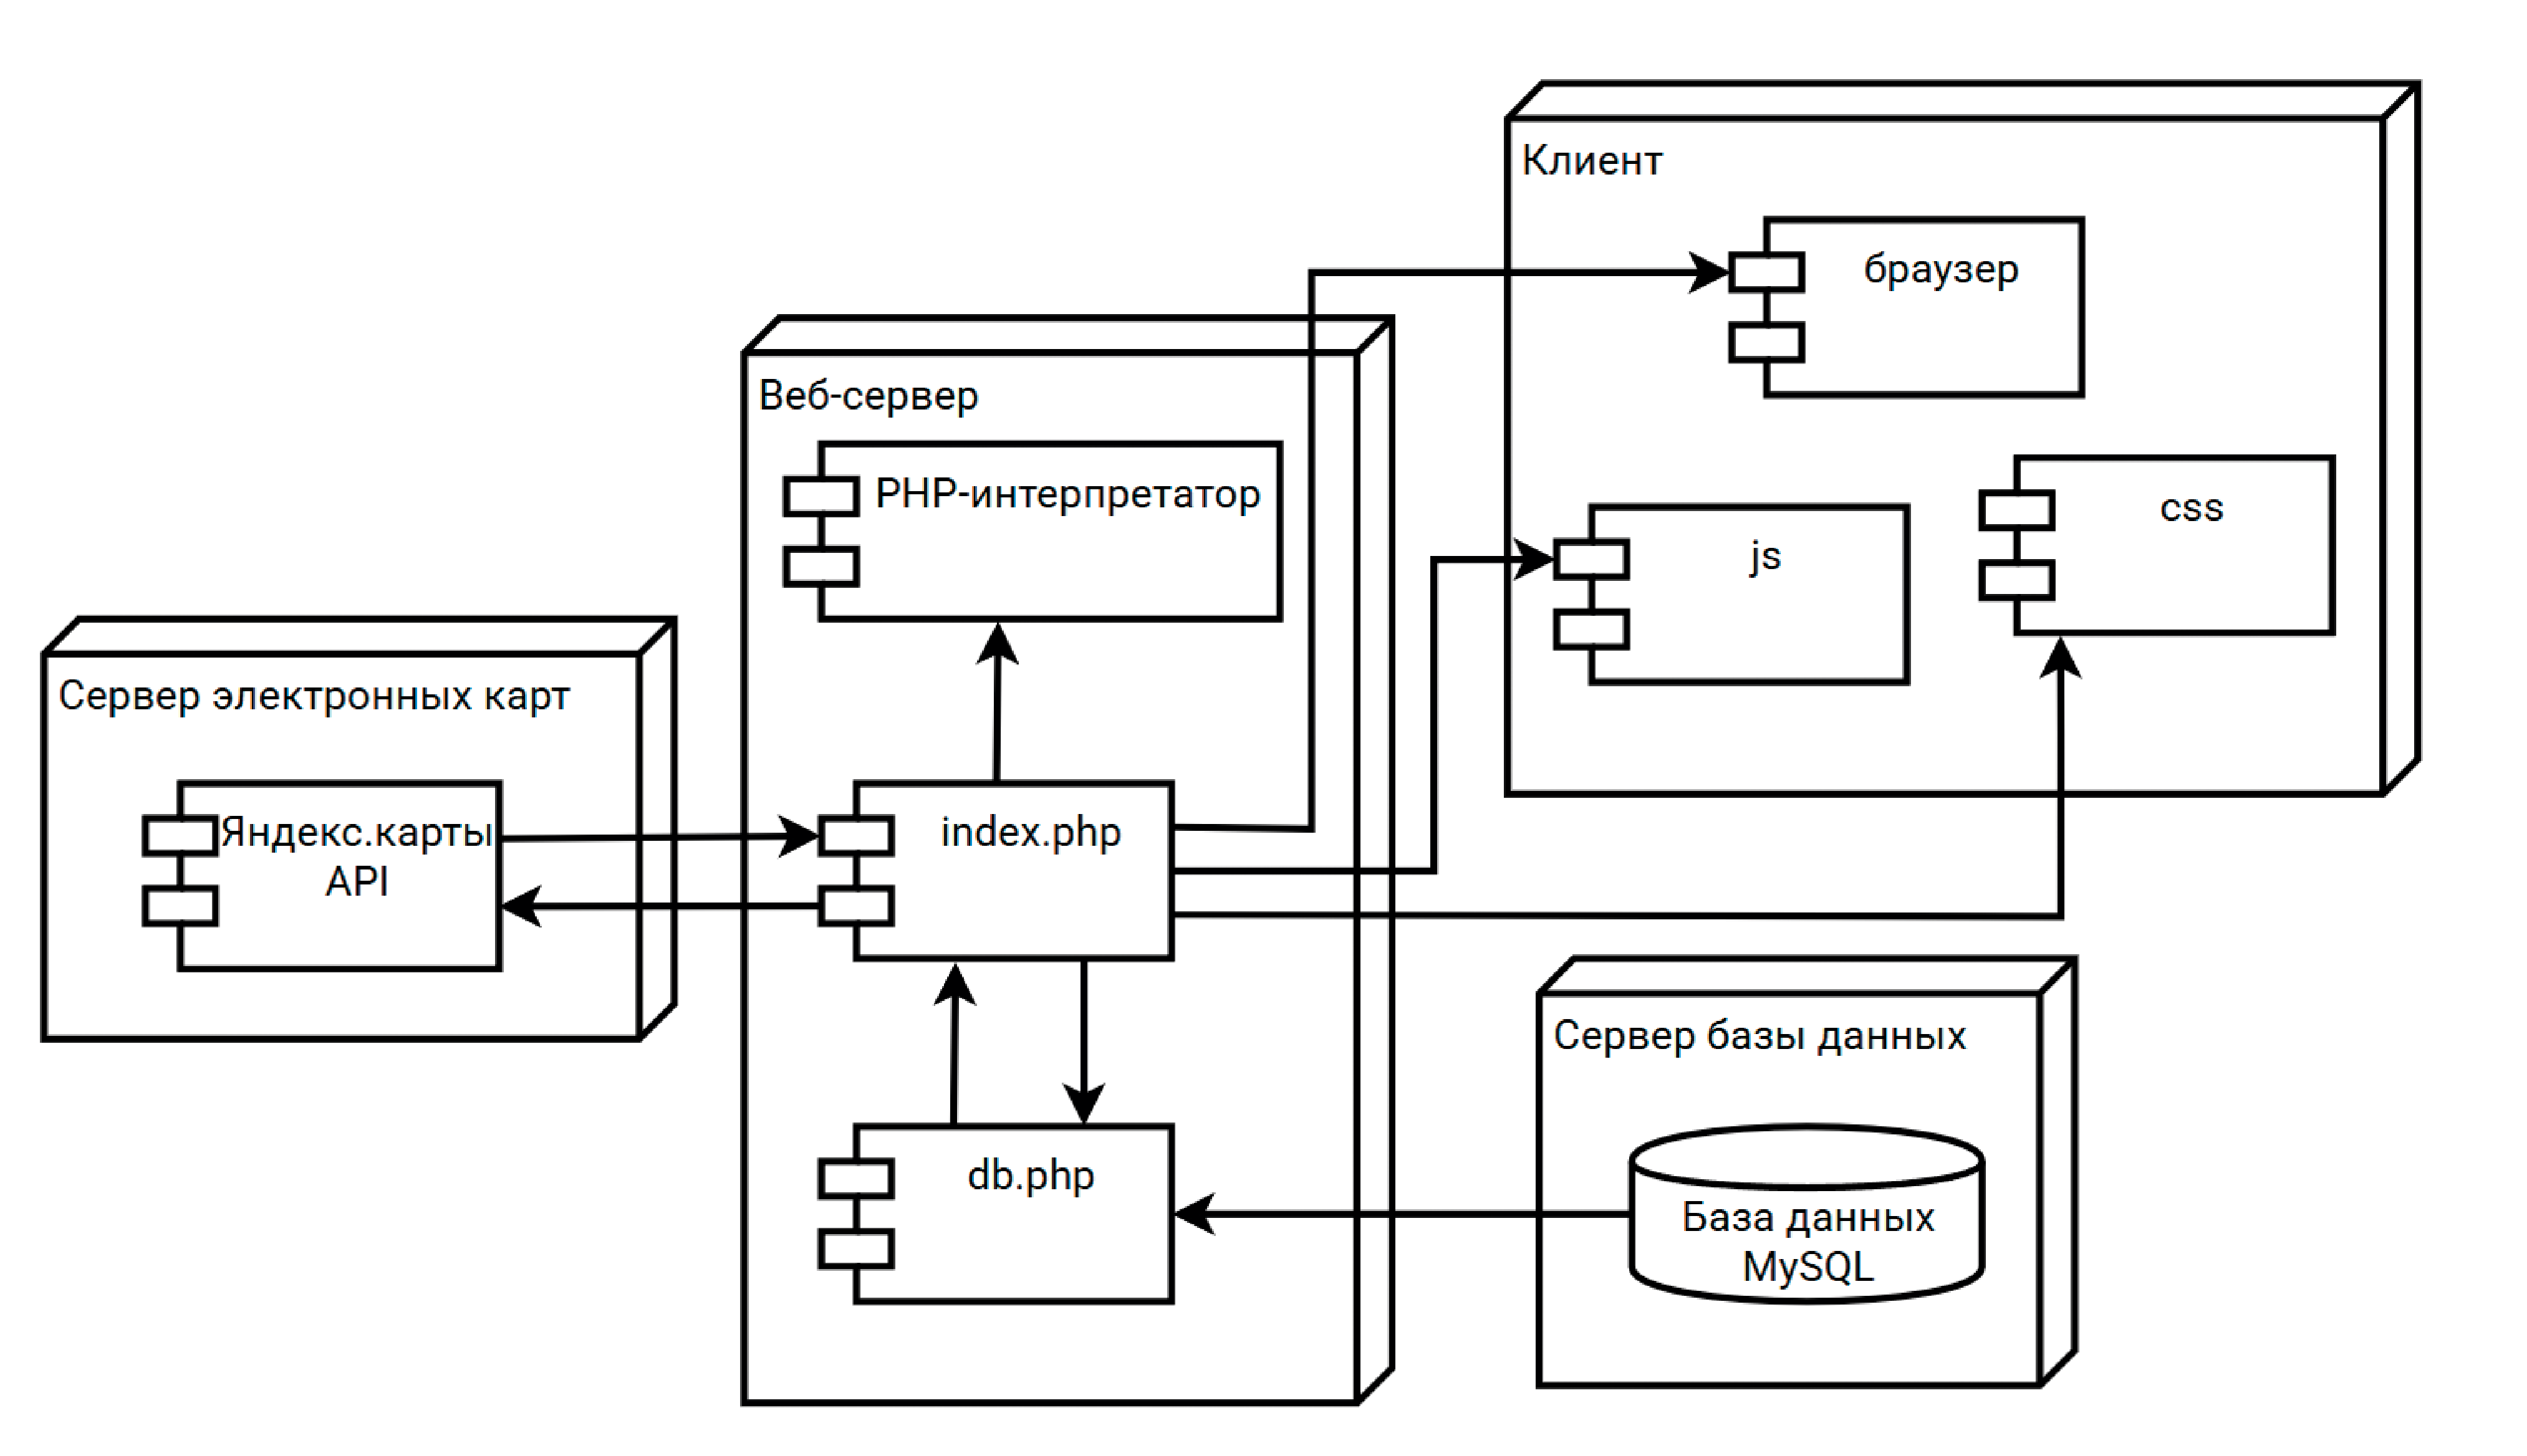
\includegraphics[width=1\linewidth]{data.png}}
	\caption{Архитектура программной системы}
	\label{data:image}
\end{figure}

\subsection{Построение маршрутов и интеграция с API Яндекс.Карт}

Одна из ключевых задач разрабатываемого веб-приложения — обеспечение функционала построения маршрутов между выбранными туристическими объектами. В отличие от стандартных навигационных систем, где путь прокладывается между двумя точками, пользователь данного приложения может создавать маршруты произвольной сложности с промежуточными остановками, сортировать порядок следования точек и выбирать предпочтительный тип передвижения. Для реализации этой функциональности используется API Яндекс.Карт — мощный инструмент, предоставляющий средства работы с геоданными, маршрутизацией и визуализацией картографической информации.

Особенности построения маршрутов. 
Построение маршрута начинается с выбора пользователем начальной точки, которая по умолчанию может быть определена автоматически через функцию геолокации. Затем пользователь добавляет любые доступные на карте объекты, при этом порядок следования можно изменять вручную, а также добавлять или удалять точки в любой момент.

На техническом уровне маршрут строится через объект ymaps.multiRouter.MultiRoute, который позволяет задать массив точек и параметры маршрута. Библиотека Яндекс.Карт производит расчет маршрута на стороне сервера, возвращая данные о длине пути, времени в пути и последовательности сегментов. Пользователь видит не только визуальное отображение маршрута на карте, но и текстовые инструкции (при активации пошагового режима), а также общую сводку по расстоянию и продолжительности.

Типы маршрутов. 
Приложение поддерживает выбор типа маршрута: пеший, автомобильный и общественный транспорт. Это реализуется через передачу параметра "type" в объект маршрута, что влияет на алгоритм расчета пути и предлагаемые траектории.

Работа с промежуточными точками. 
Одной из особенностей является возможность добавления промежуточных точек маршрута в произвольной последовательности. Пользователь может строить не только прямой путь «из точки A в точку B», но и составлять полноценный маршрут, охватывающий несколько достопримечательностей. Для этого формируется массив routePoints, содержащий все выбранные координаты. При необходимости маршрут можно реорганизовать — переставив точки местами, что приводит к пересчёту пути без перезагрузки карты.

Интерактивность и обновление. 
Маршрут пересчитывается автоматически при каждом изменении списка точек или их порядка. Это обеспечивает интерактивность и гибкость взаимодействия\cite{b15}. Пользователь может видеть, как меняется маршрут в реальном времени, что особенно важно при планировании маршрутов разной протяжённости и сложности. При этом используется минимальное количество ресурсов клиента, поскольку вычисления происходят на стороне Яндекса.

Визуализация и пользовательский интерфейс. 
Каждый маршрут сопровождается графическим отображением на карте с различными стилями оформления в зависимости от типа маршрута. Метки начальной, промежуточной и конечной точек выделяются визуально, а маршруты отображаются цветной линией. При наведении или клике пользователь может получить дополнительную информацию о точке или сегменте пути.

Таким образом, модуль маршрутизации является неотъемлемой частью веб-приложения и его основной пользовательской ценностью. Благодаря использованию API Яндекс.Карт удаётся добиться высокой точности расчётов, стабильной работы и масштабируемости, при этом интерфейс остаётся удобным даже для неподготовленного пользователя.

\subsection{Проект данных программной системы}

Разработка эффективной системы хранения и обработки информации требует чёткого проектирования структуры данных, отражающей как сущности предметной области, так и характер их взаимодействия. В данном случае речь идёт о цифровой платформе, отображающей туристические объекты региона, позволяющей пользователю формировать маршруты, оставлять отзывы и сохранять интересные места. Соответственно, проект данных опирается на ключевые сущности: объекты на карте, маршруты, пользователи, категории, отзывы и избранное. Все эти компоненты взаимосвязаны, и их модель должна обеспечивать целостность, логичность и возможность масштабирования.

Центральным элементом системы является туристический объект. Он представляет собой точку интереса, отображаемую на карте и содержащую базовую информацию: координаты, название, описание, привязку к определённой категории, а также опционально — изображения. Каждый такой объект может быть отображён на маршруте, добавлен в избранное и иметь прикреплённые отзывы.

Пользователи являются участниками системы с различным уровнем доступа. Для них предусматривается хранение учётной информации: адреса электронной почты, зашифрованного пароля, имени и роли в системе. Пользователь может быть как обычным посетителем, формирующим маршруты и просматривающим карту, так и администратором, получающим доступ к инструментам модерации. В базе данных с каждым пользователем связывается его история маршрутов и список избранных объектов.

Особое внимание уделяется маршрутам, которые пользователь может строить вручную. Структура маршрута должна быть гибкой, чтобы позволять добавление произвольного числа точек, определение порядка следования и выбор типа передвижения. Поэтому маршруты представлены двумя уровнями данных: заголовочной частью (название, тип маршрута) и набором точек маршрута. Каждая точка в маршруте включает координаты, название и, при наличии, связь с объектом из основного справочника. Дополнительно может храниться информация об адресе, полученная в процессе геокодирования, и флаг, указывающий на начальную точку.

Отдельно проектируется подсистема отзывов, позволяющая пользователям оставлять текстовые комментарии к объектам. Каждый отзыв содержит информацию об авторе, времени публикации, тексте сообщения и объекте, к которому он относится. Это позволяет в дальнейшем использовать отзывы для формирования пользовательского рейтинга, а также для отображения обратной связи в интерфейсе приложения.

Для организации и группировки объектов вводится система категорий. Каждая категория содержит идентификатор, название и визуальный признак (иконку), который используется при отображении на карте. Такая структура позволяет гибко фильтровать отображаемые точки и упрощает восприятие данных.

Существенную роль играет механизм избранного. Это логическая связь между пользователем и объектами, которые он отметил для последующего просмотра. Связь реализуется как отдельная сущность, позволяющая фиксировать не только факт добавления. Такая структура полезна при персонализации интерфейса или последующем анализе пользовательского поведения.

Вся модель данных строится с учётом реляционной логики и соблюдением принципов нормализации. Это позволяет обеспечить отсутствие дублирования информации, упрощает поддержку данных в актуальном состоянии и способствует стабильной работе при росте объёма пользователей и объектов.

Таким образом, проект данных представляет собой структурированную и логически выстроенную модель взаимодействующих сущностей, на которых основана работа веб-приложения. Он обеспечивает надёжную основу для хранения и обработки информации, поддерживает расширяемость проекта и отвечает требованиям удобства как для пользователя, так и для администратора системы.

Исходя из требований, можно выделить следующие основные сущности:

\begin{itemize}
	\item пользователи;
	\item туристические объекты;
	\item категории объектов;
	\item избранное;
	\item маршруты;
	\item точки маршрута;
	\item отзывы.
\end{itemize}

В состав сущности "<Пользователи"> можно включить атрибуты, представленные в таблице \ref{news:table}.

\begin{xltabular}{\textwidth}{|l|l|p{1.7cm}|X|}
	\caption{Атрибуты сущности "<Пользователи">\label{news:table}}\\ \hline
	\centrow Поле & \centrow Тип & \centrow Обяза\-тельное & \centrow Описание \\ \hline
	\thead{1} & \thead{2} & \centrow 3 & \centrow 4 \\ \hline
	\endfirsthead
	\continuecaption{Продолжение таблицы \ref{news:table}}
	\thead{1} & \thead{2} & \centrow 3 & \centrow 4 \\ \hline
	\finishhead
	id & Integer & true & Уникальный идентификатор пользователя \\ \hline 
	name & Varchar & true & Отображаемое имя пользователя \\ \hline 
	email & Varchar & true & Адрес электронной почты (уникальный) \\ \hline 
	password\_hash & Varchar & true & Хешированный пароль \\ \hline 
	role & Enum & true & Роль пользователя (например: user, admin)
	
\end{xltabular}

В состав сущности "<Туристические объекты"> можно включить атрибуты, представленные в таблице \ref{news:table1}.

\begin{xltabular}{\textwidth}{|l|l|p{1.7cm}|X|}
	\caption{Атрибуты  сущности "<Туристические объекты">\label{news:table1}}\\ \hline
	\centrow Поле & \centrow Тип & \centrow Обяза\-тельное & \centrow Описание \\ \hline
	\centrow 1 & \centrow 2 & \thead{3} & \centrow 4 \\ \hline
	\endfirsthead
	\continuecaption{Продолжение таблицы \ref{news:table1}}
	\centrow 1 & \centrow 2 & \thead{3} & \centrow 4 \\ \hline
	\finishhead
	id & Integer & true & Уникальный идентификатор туристического объекта \\ \hline 
	name & Varchar & true & Название объекта \\ \hline 
	description & Text & false & Краткое описание объекта \\ \hline  
	latitude & Float & true & Географическая широта объекта \\ \hline   
	longitude & Float & true & Географическая долгота объекта \\ \hline  
	category\_id & Integer & true & Идентификатор категории, к которой принадлежит объект\\ \hline  
	image\_url & Varchar & false & Ссылка на изображение объекта \\ \hline 
	created\_by & Integer & false & ID пользователя, добавившего объект \\ \hline 
	is\_active & Boolean & true & Флаг отображения объекта на карте
	
\end{xltabular}

В состав сущности "<Категории объектов"> можно включить атрибуты, представленные в таблице \ref{news:table2}.

\begin{xltabular}{\textwidth}{|l|l|p{1.7cm}|X|}
	\caption{Атрибуты  сущности "<Категории объектов">\label{news:table2}}\\ \hline
	\centrow Поле & \centrow Тип & \centrow Обяза\-тельное & \centrow Описание \\ \hline
	\centrow 1 & \centrow 2 & \thead{3} & \centrow 4 \\ \hline
	\endfirsthead
	\continuecaption{Продолжение таблицы \ref{news:table2}}
	\centrow 1 & \centrow 2 & \thead{3} & \centrow 4 \\ \hline
	\finishhead
	id & Integer & true & Уникальный идентификатор категории \\ \hline 
	name & Varchar & true & Название категории (например, Музей, Природа) \\ \hline 
	icon & Varchar & false & Путь к иконке категории для отображения на карте
		
\end{xltabular}

В состав сущности "<Избранное"> можно включить атрибуты, представленные в таблице \ref{news:table3}.

\begin{xltabular}{\textwidth}{|l|l|p{1.7cm}|X|}
	\caption{Атрибуты  сущности "<Избранное">\label{news:table3}}\\ \hline
	\centrow Поле & \centrow Тип & \centrow Обяза\-тельное & \centrow Описание \\ \hline
	\centrow 1 & \centrow 2 & \thead{3} & \centrow 4 \\ \hline
	\endfirsthead
	\continuecaption{Продолжение таблицы \ref{news:table3}}
	\centrow 1 & \centrow 2 & \thead{3} & \centrow 4 \\ \hline
	\finishhead
	user\_id & Integer & true & ID пользователя, добавившего объект в избранное \\ \hline 
	point\_id & Integer & true & ID объекта, добавленного в избранное
	
\end{xltabular}

В состав сущности "<Маршруты"> можно включить атрибуты, представленные в таблице \ref{news:table4}.

\begin{xltabular}{\textwidth}{|l|l|p{1.7cm}|X|}
	\caption{Атрибуты  сущности "<Маршруты">\label{news:table4}}\\ \hline
	\centrow Поле & \centrow Тип & \centrow Обяза\-тельное & \centrow Описание \\ \hline
	\centrow 1 & \centrow 2 & \thead{3} & \centrow 4 \\ \hline
	\endfirsthead
	\continuecaption{Продолжение таблицы \ref{news:table4}}
	\centrow 1 & \centrow 2 & \thead{3} & \centrow 4 \\ \hline
	\finishhead
	id & Integer & true & Уникальный идентификатор маршрута \\ \hline 
	user\_id & Integer & true & ID пользователя, создавшего маршрут \\ \hline 
	name & Varchar & true & Название маршрута \\ \hline 
	type & Enum & true & Тип маршрута (например, пеший, автомобильный)
	 
\end{xltabular}

В состав сущности "<Точки маршрута"> можно включить атрибуты, представленные в таблице \ref{news:table5}.

\begin{xltabular}{\textwidth}{|l|l|p{1.7cm}|X|}
	\caption{Атрибуты  сущности "<Точки маршрута">\label{news:table5}}\\ \hline
	\centrow Поле & \centrow Тип & \centrow Обяза\-тельное & \centrow Описание \\ \hline
	\centrow 1 & \centrow 2 & \thead{3} & \centrow 4 \\ \hline
	\endfirsthead
	\continuecaption{Продолжение таблицы \ref{news:table5}}
	\centrow 1 & \centrow 2 & \thead{3} & \centrow 4 \\ \hline
	\finishhead
	id & Integer & true & Уникальный идентификатор точки маршрута \\ \hline 
	route\_id & Integer & true & ID маршрута, к которому принадлежит точка \\ \hline 
	point\_id & Integer & false & ID объекта (если точка — это объект карты) \\ \hline 
	latitude & Float & false & Широта точки (если она не связана с объектом) \\ \hline 
	longitude & Float & false & Долгота точки (если она не связана с объектом) \\ \hline 
	address & Varchar & false & Адрес точки (результат геокодирования) \\ \hline 
	order\_index & Integer & true & Порядковый номер точки в маршруте
	
\end{xltabular}

В состав сущности "<Отзывы"> можно включить атрибуты, представленные в таблице \ref{news:table6}.

\begin{xltabular}{\textwidth}{|l|l|p{1.7cm}|X|}
	\caption{Атрибуты  сущности "<Отзывы">\label{news:table6}}\\ \hline
	\centrow Поле & \centrow Тип & \centrow Обяза\-тельное & \centrow Описание \\ \hline
	\centrow 1 & \centrow 2 & \thead{3} & \centrow 4 \\ \hline
	\endfirsthead
	\continuecaption{Продолжение таблицы \ref{news:table6}}
	\centrow 1 & \centrow 2 & \thead{3} & \centrow 4 \\ \hline
	\finishhead
	id & Integer & true & Уникальный идентификатор отзыва \\ \hline 
	user\_id & Integer & true & ID пользователя, оставившего отзыв \\ \hline 
	point\_id & Integer & true & ID объекта, к которому относится отзыв \\ \hline 
	content & Text & true & Текстовое содержание отзыва 
	
\end{xltabular}

\subsection{Проектирование пользовательского интерфейса}

Создание удобного и визуально сбалансированного пользовательского интерфейса\cite{b16} является одной из ключевых задач при разработке веб-приложений, ориентированных на широкую аудиторию. В контексте проекта по цифровизации туристических объектов региона особую роль играет не только функциональность интерфейса, но и его способность направлять внимание пользователя, упрощать взаимодействие с интерактивной картой и быстро предоставлять доступ к основным действиям: фильтрации, маршрутизации, просмотру информации и управлению своим профилем.

Интерфейс спроектирован таким образом, чтобы пользователю было достаточно одного экрана для выполнения большинства операций — от навигации по карте до построения маршрута. Центром внимания в приложении служит карта, отображающая туристические объекты. Остальные элементы располагаются по периферии и не перекрывают рабочую область, а открываются по необходимости: например, боковые панели, выпадающие меню и модальные окна. Такой подход обеспечивает сохранение ориентации на карте и минимизирует визуальные помехи.

Проектирование интерфейса основано на модульной структуре. Каждый элемент системы, будь то фильтр категорий, форма построения маршрута или карточка объекта, разрабатывается как самостоятельный интерфейсный блок. Это упрощает как техническую реализацию (например, переиспользование компонентов), так и восприятие для пользователя, поскольку каждое действие логически отделено и выполняется в своей зоне.

Взаимодействие с пользователем начинается с загрузки карты, на которой по умолчанию отображаются все активные туристические объекты региона. Навигация осуществляется через элементы фильтрации, позволяющие мгновенно скрывать или показывать объекты определённых категорий. При наведении на метку пользователь получает краткую информацию об объекте во всплывающем балуне, а при клике — расширенную карточку с описанием, изображением и кнопками действий (добавить в маршрут, избранное, оставить отзыв).

Отдельное внимание уделено проектированию маршрутизатора — интерфейса для построения пользовательских маршрутов. В соответствующем окне пользователь указывает начальную и конечную точки, а также может добавлять промежуточные. Система автоматически прокладывает маршрут с помощью внешнего API\cite{b17} и отображает его на карте в реальном времени. Информация о маршруте, включая продолжительность и длину, отображается в отдельной панели. Особенность реализации заключается в возможности интерактивного редактирования порядка точек, что позволяет гибко настраивать путь.

Аутентификация пользователей реализуется через минималистичную форму входа и регистрации. После авторизации появляются дополнительные элементы интерфейса. Непрерывная работа сессии и визуальное подтверждение действий (например, уведомление о добавлении в избранное) создают ощущение целостности и контроля над процессом.

Визуальный стиль интерфейса стремится к простоте и функциональной чистоте. Используются нейтральные цвета фона, акцентные кнопки. Отступы и иконки подобраны так, чтобы элементы не сливались, но и не перегружали экран. Большинство компонентов адаптированы под мобильные устройства: меню сворачиваются, форма маршрута упрощается, карта масштабируется под маленькие экраны.

Особое внимание в процессе проектирования уделено доступности\cite{b20}. Все интерактивные элементы имеют контрастную визуализацию, поддерживают навигацию с клавиатуры, а всплывающие уведомления сопровождаются альтернативным текстом. Такой подход расширяет аудиторию и соответствует современным рекомендациям по доступному веб-дизайну.

На рисунке \ref{gr1:image} представлен макет основного окна веб-приложения. Он содержит следующие элементы:

\begin{enumerate}
	\item Карта.
	\item Панель управления("<Маршрут">, "<Фильтр">, "<Создание точки">, "<Авторизация">).
	\item Метка объекта на карте.
	\item Кнопка включения и выключения геолокации.
	\item Поиск по слову.
	\item Масштаб.
\end{enumerate}

\vspace{+40mm}
\begin{figure}[ht]
	\center{
\includegraphics[width=1\linewidth]{gr1}}
	\caption{Макет интерфейса}
	\label{gr1:image}
\end{figure}

На рисунке \ref{gr7:image} представлен макет формы "<Маршрут">. Ниже показаны следующие его элементы:

\begin{enumerate}
	\item Точка маршрута.
	\item Кнопка удаления точки из маршрута.
	\item Кнопка для добавления маршрута в избранное.
	\item Кнопки для переключения типа маршрута.
	\item Кнопка для оптимизации маршрута.
	\item Информация о длине и примерном времени маршрута.
	\item Кнопка включения и выключение подробным инструкций.
	\item Пошаговые инструкции.
	\item Кнопки закрытия формы без очистки маршрута.
	\item Кнопка закрытия формы и очистки маршрута.
\end{enumerate}

\begin{figure}[ht]
	\center{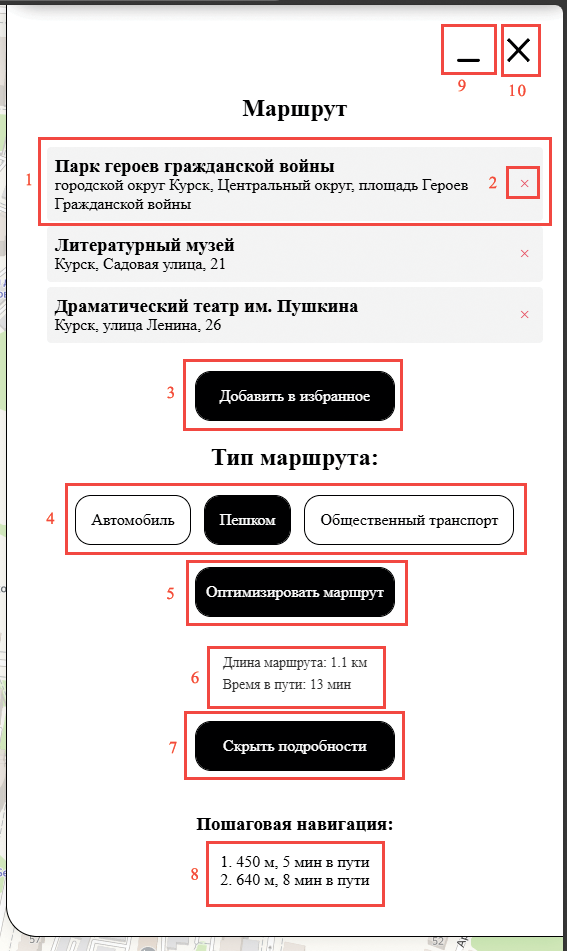
\includegraphics[width=0.5\linewidth]{gr7}}
	\caption{Макет интерфейса "<Маршрут">}
	\label{gr7:image}
\end{figure}

На рисунке \ref{gr4:image} представлен макет формы "<Фильтр">. Макет содержит следующие элементы:

\begin{enumerate}
	\item Кнопки закрытия формы.
	\item Флаги включения и выключения отображения типов объектов на карте.
\end{enumerate}

\vspace{+80mm}
\begin{figure}[ht]
	\center{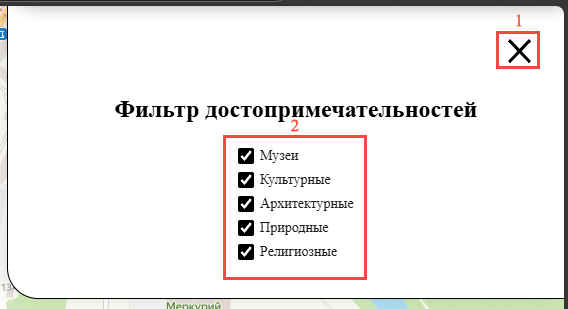
\includegraphics[width=1\linewidth]{gr4}}
	\caption{Макет интерфейса "<Фильтр">}
	\label{gr4:image}
\end{figure}

На рисунке \ref{gr5:image} представлен макет формы "<Создание точки">. Он содержит следующие элементы:

\begin{enumerate}
	\item Поле ввода названия.
	\item Адрес точки.
	\item Список для выбора категории.
	\item Кнопки подтверждения.
	\item Расположение метки на карте.
	\item Кнопка закрытия формы.
\end{enumerate}

\vspace{+80mm}
\begin{figure}[ht]
	\center{
\includegraphics[width=1\linewidth]{gr5}}
	\caption{Макет интерфейса "<Создание точки">}
	\label{gr5:image}
\end{figure}

На рисунке \ref{gr8:image} представлен макет формы "<Авторизация"> в случае, если пользователь еще не был зарегистрирован. Ниже показаны следующие его элементы:

\begin{enumerate}
	\item Поле ввода псевдонима.
	\item Поле ввода электронной почты.
	\item Поле ввода пароля.
	\item Поле подтверждения пароля.
	\item Кнопка подтверждения.
	\item Кнопка перехода в форму входа.
	\item Кнопка закрытия формы.
\end{enumerate}

\vspace{+40mm}
\begin{figure}[ht]
	\center{
\includegraphics[width=1\linewidth]{gr8}}
	\caption{Макет интерфейса "<Авторизация">. Пользователь регистрируется впервые.}
	\label{gr8:image}
\end{figure}

На рисунке \ref{gr9:image} представлен макет формы "<Авторизация"> в случае, когда пользователь вошел в личный кабинет. Макет содержит следующие элементы:

\begin{enumerate}
	\item Список избранных мест.
	\item Список избранных маршрутов.
	\item Избранное место.
	\item Кнопка удаления из избранного.
	\item Кнопка выхода из личного кабинета.
	\item Кнопка закрытия формы.
\end{enumerate}

\begin{figure}[ht]
	\center{
\includegraphics[width=1\linewidth]{gr9}}
	\caption{Макет интерфейса "<Авторизация">. Личный кабинет пользователя.}
	\label{gr9:image}
\end{figure}

\subsection{Компоненты пользовательского интерфейса}

Пользовательский интерфейс веб-приложения является основной точкой взаимодействия между пользователем и системой, и именно JavaScript играет ключевую роль в обеспечении его интерактивности, динамики и адаптивности. В рамках разработки интерфейса применяются клиентские сценарии, реализующие управление меню, отображение и скрытие блоков, работу с объектами на карте, фильтрацию, построение маршрутов и взаимодействие с пользовательскими действиями.

Архитектура интерфейсной логики организована модульно — каждый функциональный блок представлен отдельным JavaScript-файлом, отвечающим за строго определённый участок поведения интерфейса. Такой подход обеспечивает не только читаемость и расширяемость кода, но и способствует масштабируемости проекта при добавлении новых функций.

Одним из базовых компонентов интерфейса является система управления контекстными меню — такими как «Добавить объект», «Фильтр», «Авторизация» или «Маршрут». Каждое меню реализовано через скрытые DOM-элементы, которые динамически активируются при клике на соответствующие кнопки навигации. Скрипты, такие как openAddMenu.js, openFilterMenu.js и openRegistrationMenu.js, отвечают за установку видимости и переключение состояния классов элементов, в том числе добавление или удаление стилей, а также блокировку фонового взаимодействия.

Фильтрация объектов по категориям реализована через компонент Filter.js, который прослушивает изменение состояния чекбоксов и в зависимости от выбранных значений изменяет видимость точек на карте. Это достигается путём удаления объектов с карты через методы API Яндекс.Карт.

Интерактивная работа с картой, в том числе построение маршрутов, добавление точек в избранное, отображение балунов с данными — реализуется в модулях routeHandler.js, favoritePoint.js, addReview.js и addObjectInformation.js. При взаимодействии пользователя с элементами карты или балуна инициируются события, обрабатываемые JavaScript-обработчиками. Например, при нажатии на кнопку «Добавить в маршрут» информация о точке сохраняется в массив routePoints, после чего вызывается функция пересчёта маршрута и его отображения на карте.

Особое внимание уделено работе с асинхронными данными. Для этого используются функции загрузки точек (addData.js), избранного (loadFavoritesPoints.js), отзывов (addReview.js) и маршрутов (loadFavoritesRoutes.js). JavaScript в этих случаях выполняет асинхронные запросы к серверу (fetch) и обновляет DOM без перезагрузки страницы, обеспечивая плавную и отзывчивую работу интерфейса.

Добавление отзывов реализовано через форму, события которой перехватываются с помощью JS. После валидации данных выполняется POST-запрос, и при успешной отправке отзыв добавляется в DOM-дерево страницы без необходимости повторной загрузки. Аналогичная логика применяется к добавлению объектов, их описаний и изображений.

Скрипт Location.js реализует функциональность отображения текущего положения пользователя на карте с использованием navigator.geolocation. При активации кнопки геолокации создаётся объект Placemark, который добавляется на карту, а при повторном нажатии — удаляется. Это позволяет пользователю быстро определить своё положение относительно туристических объектов.

Работа интерфейса тесно связана с данными, загружаемыми в формате JSON. JavaScript-модули используют DOM API, добавляют элементы на карту или в интерфейс, отслеживают действия пользователя и обновляют состояние приложения.

Благодаря активному использованию событийной модели, модульной архитектуре и средствам асинхронной загрузки JavaScript позволяет реализовать живой, гибкий и удобный интерфейс, который реагирует на действия пользователя немедленно, без перегрузки или визуальных задержек. Это создаёт ощущение полнофункционального приложения, при том что основная обработка осуществляется на стороне клиента.

Таким образом, JavaScript выступает как движущая сила интерфейса: он не просто дополняет верстку, а полностью формирует поведение интерфейса, поддержку пользовательского взаимодействия и связку с картографическим функционалом. Без него веб-приложение теряет свою динамичность и интерактивность, а взаимодействие пользователя с системой становится ограниченным.